\section{Policy configuration}\label{sect:seapp_config}

In this section, we explore the structure of application policy
modules.  Before describing the content of \seapp configuration files,
we give a short description of how \sea defines the security contexts
of processes, files and system services.  There are strong
similarities between the structure of system and app policies.
Indeed, we designed our solution as a natural extension of the
approach used to protect the system.  Also, our design maintains full
backward compatibility.  Developers who are not interested in taking
advantage of MAC capabilities do not have to change their apps.


\subsection{\sea policy structure}\label{sect:seapp_seandroid}

Compared to a traditional Linux implementation, Android expands the
set of configuration files where \sel~\cite{seapp_sea_files} security
contexts are described, because a wider set of entities is supported.
\sea complements the common \sel files (i.e., \filecontexts and
\genfscontexts) with 4 additional ones: \propertycontexts,
\servicecontexts, \seappcontexts and \macpermissions.  Also, the
implementation of the \sel library (\libselinux)
\cite{seapp_libselinux} has been modified introducing new functions
(to assign domains to app processes and types to their dedicated
directory).  We concisely describe the role of \sea context files.

\subsubsection{Processes}

With reference to app processes, Android assigns the security context
based on the class the app falls in.  The specification of the classes
and their security labels are defined in the \seappcontexts policy
file.  Most classes state two security contexts: one for the process
({\tt domain} property) and the other one for the app dedicated
directory ({\tt type} property).  A number of {\em input selectors}
determine the association of an app with a class.  Among these,
\seinfo filters on the tag associated with the X.509 certificate used
by the developer to sign the app.  The mapping between the certificate
and the \seinfo tag is achieved by the \macpermissions configuration
file.  Since the enumeration of all third-party app certificates is
not possible a priori, all third-party apps are labeled with the
\untrustedapp domain by default.


\subsubsection{Files}

\sel splits the configuration of security contexts of files between
\filecontexts and \genfscontexts, with the former used with
filesystems that support extended file attributes (e.g., \data), while
the latter with the ones that do not (e.g., \proc).  To apply
\filecontexts updates, two approaches are available: either rebuild
the filesystem image, or run \restorecon operation on the file or
directory to be relabeled (this is the default method used by
permissioned system processes).  Conversely, to apply \genfscontexts
changes, a reboot of the device or a sequence of filesystem {\em
  un-mount} and {\em mount} operations has to be performed.

\subsubsection{Services}

Unlike what happens for system processes, a system service requires
the assignment of a security context to both its processes and its
\binder~\cite{seapp_binder}, to be fully compliant with \sea.  The
\binder is the lightweight inter-process communication primitive
bridging access to a service.  Its retrieval is enabled by the
\servicemanager, a process started during device boot-up to keep track
of all the services available on the device.  Based on the labels
specified in the \servicecontexts file, it is then possible to control
which processes can register ({\em add}) and lookup ({\em find}) a
\binder reference for the service, and therefore connect to it.
However, since \binder handles resemble tokens with almost
unconstrained delegation, denying a process to get the \binder through
the \servicemanager does not prevent the process from obtaining it by
other means (e.g., by abusing other processes that already hold it).
Furthermore, preventing a process from obtaining a \binder reference
prevents the process from using any functionality exposed by the
service.

\subsection{\seapp policy structure}\label{subsect:seapp_structure}

Developers interested in taking advantage of our approach to improve
the security of their apps are required to load the policy into their
Android Package (APK).  A predefined directory, \apkpolicydir, at the
root of the archive, is where the \seapp-aware package installer will be
looking for the policy module (see
Figure~\ref{fig:seapp_policy_folder}).  Inside this directory, the
installer looks for four files (which we refer to as {\em local}),
that outline a policy structure similar to the one of the system.
Specifically, the developer is able to operate at two different
levels: (i) the actual definition of the app policy logic using the
policy language described in Section \ref{sect:seapp_lang} (in the
local file \sepolicy), and (ii) the configuration of the {\em security
  context} for each process (in the local files \seappcontexts and
\macpermissions) and for each file directory (in the local file
\filecontexts).

\begin{figure}[t]
	\centering
	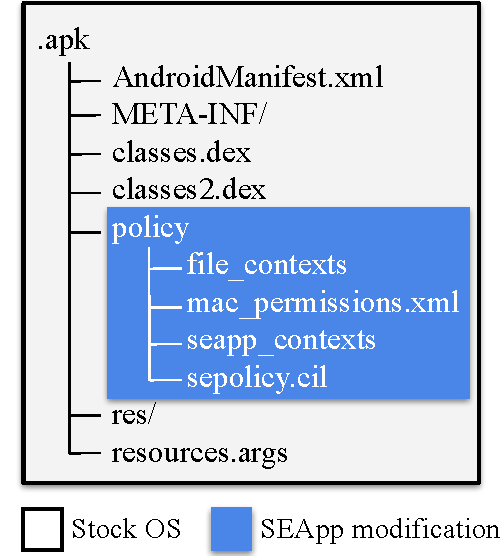
\includegraphics[width=0.4\textwidth]{chapters/seapp/figs/policy_folder}
	\caption{\seapp policy structure}
	\label{fig:seapp_policy_folder}
\end{figure}

\subsubsection{Processes}\label{subsub:seapp_process_control}

\seapp permits to assign a \sel domain to each process of the security
enhanced app.  To do this, the developer lists in the local
\seappcontexts a set of entries that determine the security context to
use for its processes.  For each entry, we restrict the list of valid
input selectors to {\tt user}, {\tt seinfo} and {\tt name}: {\tt user}
is a selector based upon the type of UID; {\tt seinfo} matches the app
seinfo tag contained in the local \macpermissions configuration file;
{\tt name} matches either a prefix or the whole process name.  The
conjunction of these selectors determines a class of processes, to
which the context specified by {\tt domain} is assigned.  To avoid
privilege escalation, the only permitted domains are the ones the app
defines within its policy module and \untrustedapp. As a process may
fall into multiple classes, the most selective one, with respect to
the input selector, is chosen.  An example of valid local
\seappcontexts entries is shown in Listing~\ref{seapp_lstseapp}, which
shows the assignment of the {\em unclassified} and {\em secret}
domains to the {\em :unclassified} and {\em :secret} processes,
respectively.

In Android, developers have to focus on components rather than
processes.  Normally, all components of an application run in a single
process.  However, it is possible to change this default behavior
setting the \texttt{android:process} attribute of the respective
component inside the \manifest, thus declaring what is usually called
a {\em remote} component.  Furthermore, with the specification of an
\texttt{android:process} consistent with the local \seappcontexts
configuration, we support the assignment of distinct domains to app
components.  To execute the component, the developer is only required
to create the proper \emph{Intent} object~\cite{seapp_intentsstart},
as she would have already done on stock Android for remote components.
The assignment to the process of the correct domain is handled by the
system.  This design choice allows us to support Android activities,
services, broadcast receivers and content providers, while avoiding
changes to the \textit{PackageParser}~\cite{seapp_packparse}, as there
are no modifications to the manifest schema.

\subsubsection{Files}\label{subsub:seapp_files_control}

The developer states the \sel security contexts of internal files in
the local \filecontexts.  Each of its entries presents three syntactic
elements, \texttt{pathname\textunderscore regexp},
\texttt{file\textunderscore type} and \texttt{security\textunderscore
  context}: \texttt{pathname\textunderscore re}- \newline {\tt gexp}
defines the directory the entry is referred to (it can be a specific
path or a regular expression); \texttt{file\textunderscore type}
describes the class of filesystem resource (i.e., directory, file,
etc.); \texttt{security\textunderscore context} is the security
context used to label the resource.  The admissible entries are those
confined to the app dedicated directory and using types defined by the
app policy module, with the exception of \appdatafile.  Due to the
regexp support, a path may suit more entries, in which case the most
specific one is used.  Examples of valid local \filecontexts entries
are shown in Listing~\ref{seapp_lstfile}: the first line describes the
default label for app files, second and third line respectively
specify the label for files in directories {\tt dir/unclassified} and
{\tt dir/secret}.

In \sel, the security context of a file is inherited from the parent
folder, even though \filecontexts might state otherwise.  Since, for
our approach, it is essential that files are labeled as expected by
the developer, we decided to enforce file relabeling at creation.
Therefore, a new native service has been added to the system (see
Section~\ref{sect:seapp_app_runtime}).  We then offer to the developer an
alternative implementation of class \texttt{java.io.File}, named
\texttt{android.os.File}, which sets file and directory context upon
its creation, transparently handling the call to our service.


\subsubsection{System services}\label{subsub:seapp_service_control}

To support any third-party app, the \untrustedapp domain grants to a
process the permissions to access all system services an app could
require in the \manifest.  As an example, in Android 11, the
\texttt{untrusted\textunderscore ap}- \newline {\tt p\textunderscore
  all.te} platform policy file~\cite{seapp_untrustedappte} permits to
a process labeled with {\tt untrusted}- \newline {\tt \textunderscore
  app} to access \texttt{audioserver}, \texttt{camera},
\texttt{location}, \texttt{mediaserver}, \texttt{nfc} services and
many more.

To prevent certain components of the app from holding the privilege to
bind to unnecessary system services, the developer defines a domain
with a subset of the \untrustedapp privileges (in the local \sepolicy
file), and then she ensures the components are executed in the process
labeled with it.  Listing~\ref{seapp_lstdomains} shows an example in
which the {\tt cameraserver} service is made accessible to the {\em
  secret} process.  \newline
\begin{lstlisting}[language=policyfile, caption=\seappcontexts
example, captionpos=b, label=seapp_lstseapp, numbersep=2pt,resetmargins=false]
 user=_app seinfo=cert_id domain=package_name.unclassified name=package.name:unclassified
 user=_app seinfo=cert_id domain=package_name.secret name=package.name:secret
\end{lstlisting}
%
\begin{lstlisting}[language=policyfile, caption=\filecontexts
example, captionpos=b, label=seapp_lstfile, numbersep=2pt,resetmargins=false]
 .*                u:object_r:app_data_file:s0
 dir/unclassified  u:object_r:package_name.unclassified_file:s0
 dir/secret        u:object_r:package_name.secret_file:s0
\end{lstlisting}
%
\begin{lstlisting}[language=policyfile, caption=Granting \texttt{cameraserver}
access to secret domain, captionpos=b, label=seapp_lstdomains, numbersep=2pt,resetmargins=false]
(block package_name
  (type secret)
  (call md_appdomain (secret))
  (typebounds untrusted_app secret)
  (allow secret cameraserver_service (service_manager (find)))...)
\end{lstlisting}

%%% Local Variables: 
%%% mode: latex
%%% TeX-master: "../../../main.tex"
%%% reftex-default-bibliography: "../../../bib/biblio.bib"
%%% End: